\chapter{Implementation}
\label{sec:implementation}

% Hier greift man einige wenige, interessante Gesichtspunkte der
% Implementierung heraus. Das Kapitel darf nicht mit Dokumentation oder
% gar Programmkommentaren verwechselt werden. Es kann vorkommen, daß
% sehr viele Gesichtspunkte aufgegriffen werden müssen, ist aber nicht
% sehr häufig. Zweck dieses Kapitels ist einerseits, glaubhaft zu
% machen, daß man es bei der Arbeit nicht mit einem "Papiertiger"
% sondern einem real existierenden System zu tun hat. Es ist sicherlich
% auch ein sehr wichtiger Text für jemanden, der die Arbeit später
% fortsetzt. Der dritte Gesichtspunkt dabei ist, einem Leser einen etwas
% tieferen Einblick in die Technik zu geben, mit der man sich hier
% beschäftigt. Schöne Bespiele sind "War Stories", also Dinge mit denen
% man besonders zu kämpfen hatte, oder eine konkrete, beispielhafte
% Verfeinerung einer der in Kapitel 3 vorgestellten Ideen. Auch hier
% gilt, mehr als 20 Seiten liest keiner, aber das ist hierbei nicht so
% schlimm, weil man die Lektüre ja einfach abbrechen kann, ohne den
% Faden zu verlieren. Vollständige Quellprogramme haben in einer Arbeit
% nichts zu suchen, auch nicht im Anhang, sondern gehören auf Rechner,
% auf denen man sie sich ansehen kann.

%\ldots implementation \ldots

The chapter outlines the implementation of the system designed in Chapter~\ref{sec:design}. Firstly, it illustrates the implementation of the attestation and provisioning infrastructure (Section~\ref{sec:impl_attestation_infr}). This includes the communication establishment between the 
attestation and provisioning agent with the secret manager, the way the secret injector deploys secrets, the runtime attestation support's implementation, and how the attestation driver acquires attestation reports from \acrshort{TEE}. Secondly, it details the implementation of the 
software measurement manager (~\ref{sec:impl_measurement}). Section~\ref{sec:impl_exec} then presents the EXEC checker's steps for checking an exec request. Finally, sections~\ref{sec:impl_STDIO},~\ref{sec:impl_interceptor}, and~\ref{sec:iml_qlog} explain the implementation of the process's STDIO 
protection, system call interceptor, and the Qkernel log manager, respectively. The source code is accessible on GitHub~\cite*{theis_source_code}.

\section{Attestation and Provisioning Infrastructure}
\label{sec:impl_attestation_infr}

\subsection{Secret Uploading}
The secret manager must operate within the application owner's local environment. It implements a local file system backend. The application owner can deploy secrets to a path the secret manager can find using a script~\cite*{secret_uploading_script}. The functionality to create a secure channel 
based on TLS~\cite*{tls_record_size} and attestation and then upload secrets still needs to be implemented.

\subsection{Attestation and Provisioning Agent}
The attestation and provisioning agent is a HTTPS client designed to provide the \acrshort{CVM} with the following interface to prove its identity to the secret manager and fetch secrets.

\begin{lstlisting}[language=rust, caption= API of the atestation and provisioning agent]
    pub fn provisioning_http_client(task: &Task, software_maasurement: &str, sm_cert: Vec<u8>) -> Result<(KbsPolicy, KbsSecrets)>
\end{lstlisting}

The function takes the shield startup hash and the secret manager’s public key as arguments and returns the shield policy and application’s secrets if attestation succeeds. Note that this function is called only after loading the application binary because the shield startup hash is 
generated afterward. This function solves the following three problems:

\begin{enumerate}
    \item How the agent establishes a TCP connection to the secret manager
    \item How the agent establishes a TLS channel on top of the TCP connection to the secret manager
    \item How the agent constructs HTTP requests according to the KBS attestation protocol, proves its identity to the secret manager, and retrieves secrets.
\end{enumerate}

\subsubsection{TCP connection establishment}

Listing~\ref{lst:api_for_tcp_connection} shows the API for establishing the TCP connection. In order to make the Qkernel socket object available to the shield layer, the \emph{Provider} interface defined in the Qkernel network stack is implemented for the \emph{ShieldSocketProvider}. Since each 
socket implements trait \emph{SockOperations}, the shielding layer can first use \emph{ShieldSocketProvider} to obtain a socket object and then use \emph{Connect()} method to connect the socket to the secret manager.

\begin{lstlisting}[language=rust, caption= API for establishing the TCP connection, label={lst:api_for_tcp_connection}]
pub struct ShieldSocketProvider {
    pub family: i32,
}

impl Provider for ShieldSocketProvider {
    fn Socket(...) -> Result<Option<Arc<File>>>;
}

pub trait SockOperations: Sync + Send {
    fn Connect(...) -> Result<i64> {}
…
}    
\end{lstlisting}

\subsubsection{TLS channel establishment}
Listing~\ref{lst:api_for_tls_connection} shows the functions for creating a TLS channel. The no-std compatible crate embedded-tls~\cite*{embede_tls} is used to establish a TLS channel between the secret manager and the \acrshort{CVM}, as the guest kernel (Qkernel) runs in a no-std environment. The 
socket connected to the secret manager is stored in \emph{ShieldProvisioningHttpSClient}. Therefore, the \emph{ShieldProvisioningHttpSClient} implements the traits \emph{embedded\_io::blocking::Read} and \emph{embedded\_io::blocking::Write}. The embedded-tls library can then use the functions 
in these two traits to read and write the socket stored in \emph{ShieldProvisioningHttpSClient}.

\begin{lstlisting}[language=rust, caption= API for establishing the TLS channel, label={lst:api_for_tls_connection}]
pub struct ShieldProvisioningHttpSClient {
    pub socket_file: Arc<File>,
    ...
}

impl embedded_io::blocking::Read for ShieldProvisioningHttpSClient {
    fn read<'m>(&'m mut self, read_to: &'m mut [u8]) -> Result<usize>;
}

impl embedded_io::blocking::Write for ShieldProvisioningHttpSClient {
    fn write<'m>(&'m mut self, write_from: &'m [u8]) -> Result<usize>;
}
\end{lstlisting}
\subsubsection{Building HTTP requests according to the KBS attestation protocol}
Listing~\ref{lst:http_connection} shows the functions for constructing the HTTP requests defined in the KBS attestation protocol~\cite*{kbs_Attestation_protocol}. \emph{ShieldProvisioningHttpSClient} holds the metadata used in the protocol. The explanation of those data can be found in 
section~\ref{sec:kbs};


The functions \emph{prepair\_post\_auth\_http\_req}, \emph{prepair\_post\_attest\_http\_req}, and \emph{prepair\_get\_resource\_http\_req} are employed to construct the HTTP request string defined in the KBS attestation protocol, i.e., \texttt{Post /kbs/v0/auth}, \texttt{Post /kbs/v0/attest}, and
\texttt{GET /kbs/v0/<resource\_id>}. 
The generated string is submitted to the embedded-tls library~\cite*{embede_tls} by the function \emph{send\_http\_request\_to\_sm}. The embedded-tls library wraps the string into a TLS record and writes it to the socket stored in \emph{ShieldProvisioningHttpSClient} via the 
\emph{embedded\_io::blocking::Write} function. When the secret manager receives the request, it processes the request accordingly and returns the response, which is encapsulated in a TLS record. The embedded-tls library reads the record through the 
\emph{embedded\_io::blocking::Read} function, then decrypts it.

The decrypted string is parsed by \emph{parse\_auth\_http\_resp}, \emph{parse\_attest\_http\_resp}, or \emph{parse\_http\_get\_resource\_resp}. These functions first interpret the string according to the HTTP specification. They will then process the HTTP 
response according to the semantics of the KBS attestation protocol~\cite*{kbs_Attestation_protocol}. Specifically, for an HTTP response to \texttt{Post /kbs/v0/auth}, function \emph{parse\_auth\_http\_resp} will save the cookie and nonce to \emph{ShieldProvisioningHttpSClient}. 
For \texttt{Post /kbs/v0/attest}'s response, the \emph{parse\_attest\_http\_resp} function will check HTTP response status codes to determine if the attestation is successful. When a \texttt{GET /kbs/v0/} response is received, the \emph{parse\_http\_get\_resource\_resp} function is called. 
It decrypts the payload using the private part of \emph{tee\_key}, and returns the secret.

Furthermore, the \emph{generate\_evidence} function is invoked by the \emph{prepair\_post\_attest\_http\_req} when generating the \texttt{Post /kbs/v0/attest} request string. It prompts the attestation driver to produce an attestation report. The custom field of the report includes the 
hash of the nonce, the public part of the \emph{tee\_key}, and the shield's startup hash.                                                                                                                                                                                                                                                                                                


\begin{lstlisting}[language=rust, caption= Functions for building the HTTP requests defined in the KBS attestation protocol, label={lst:http_connection}]
fn send_http_request_to_sm (...)->  core::result::Result<… >;

pub struct ShieldProvisioningHttpSClient {
    pub socket_file: Arc<File>,
    cookie: String,
    nonce: String,
    tee_key: Option<TeeKey>,
    pub tee_type: Tee,
}

impl ShieldProvisioningHttpSClient {
    fn prepair_post_auth_http_req(&self) -> String;
    fn parse_auth_http_resp(&mut self, resp_buf: &[u8]) -> Result<()>;
    fn prepair_post_attest_http_req(&self, software_maasurement: &str) -> Result<String>;
    fn parse_attest_http_resp(&mut self, resp_buf: &[u8]) -> Result<()>;
    fn prepair_get_resource_http_req(&self, resource_url: String) -> String;
    fn parse_http_get_resource_resp(&mut self, resp_buf: &[u8]) -> Result<Vec<u8>>;
    fn generate_evidence(&self, software_maasurement: &str) -> Result<Attestation>;
}
    
\end{lstlisting}

It is important to note that HTTP requests and responses alike are bound within a strict 16 KB limit, as the maximum TLS record size is 16 KB~\cite*{tls_record_size}. Inevitably, the secret size is also subject to the 16 KB limit. Since file type secrets can be huge, the 
shield must execute a single HTTP GET request for each file. Generally speaking, the application owner may inject a shield policy, a file containing environment variables and command line arguments of the application, and n file type secrets into the \acrshort{CVM}. 
In this case, the shield needs to execute n+2 HTTP get requests.

\subsubsection{Limitations}
\label{subsec:Limitations}

The attestation report is a simulated report because the Qkernel cannot operate within a \acrshort{TEE}. Upon receipt of a \texttt{POST /kbs/v0/attest} request, the secret manager will omit to verify the report signatures and \acrshort{TEE} hardware's measurements for the VM startup. 
This means the secret manager will not validate the report's genuineness and the integrity of the Qkernel binary. Furthermore, the secret manager cannot identify a \acrshort{CVM} by examing the \acrshort{CVM} id in the host data fields of the report since there is no efficient way to pass the \acrshort{CVM}
ID to the Qvisor before starting the guest. As a result, the secret manager only validates the custom field in the report, which includes the hash of the nonce, the public part of the \emph{tee\_key}, and the shield's startup hash. This ensures that the shield startup hash is consistent with the 
reference hash provided by the application owner. Identifying the \acrshort{CVM} identity, checking the report's signature, and verifying the \acrshort{TEE}'s measurement are left for future implementation.


\subsection{Secret Injector}
The secret injector keeps application secrets and deploys file-type secrets. It has the following API. 
\begin{lstlisting}[language=rust, caption= API for Secret Injector, label={lst:Secret_injector}]
pub struct SecretKeeper {
    pub secrets_mount_info: FileSystemMount,
    pub file_secrets:  BTreeMap<String, Vec<u8>>,  // key: file name, value: secret
    pub arg_env_based_secrets: Option<EnvCmdBasedSecrets>,
}

impl SecretKeeper {
    pub fn set_secrets_mount_info (&mut self, info: FileSystemMount) -> Result<()>
    pub fn bookkeep_secrets (&mut self, secrets: KbsSecrets) -> Result<()>
    pub fn inject_file_based_secret_to_secret_file_system (&self, task: &Task) -> Result<()>
}   
\end{lstlisting}

Function \emph{set\_secrets\_mount\_info} records information about the application's file system, which can be used to create a sub-filesystem for the file type secrets. As discussed in Section~\ref{sec:design_Quark_Attestation_and_Provisioning_Infrastructure}, the file system is mounted under 
directory \textbf{/secret}. Mounting the file system is facilitated by the function \emph{inject\_file\_based\_secret\_to\_secret\_file\_system}, which calls the function \emph{MountSubmounts} in Qkernel. The function \emph{bookkeep\_secrets} stores the application's secrets in the \emph{SecretKeeper}. 
Additionally, since the command-line and environment variable type secrets are pushed onto the application's stack,  \emph{SecretKeeper} does not implement any function to deploy these types of secrets.

\subsubsection{Secret Sub-filesystem}
Listing~\ref{lst:sub_filesystem} presents the API for creating the filesystem for file type secrets. \emph{SecretFileSystem} implements the  Qkernel's filesystem interface, which can be called by the \emph{mountSubmounts()} to mount the file secrets to this sub-filesystem.  During this process, 
the \emph{Mount} function creates an inode for each file type secret stored in \emph{SecretKeeper} and saves it in a BTreeMap called \emph{contents}. The BTreeMap is used to initialize the Qkernel object \emph{Dir}, which represents the directory object in Qkernel. \emph{Dir} is then used to 
initialize the inode representing the sub-filesystem, i.e., \emph{NewSecretInode}. Later, \emph{MountSubmounts} will add this inode to the \emph{mounts} fields in the structure\emph{ MountNsInternal}, which stands for the application process mount namespace.

\begin{lstlisting}[language=rust, caption= API for secret file system, label={lst:sub_filesystem}]
pub struct SecretFileSystem {}
impl Filesystem for SecretFileSystem {
    fn Mount(&mut self, task: &Task, device: &str, flags: &MountSourceFlags, data: &str) -> Result<Inode> {
            ...
    }
}

pub struct MountNsInternal {
    pub mounts: QMutex<BTreeMap<u64, Arc<QMutex<Mount>>>>,
    ...
}
      
\end{lstlisting}

The \emph{Dir} and the \emph{NewSecretInode} object implement the Qkernel \emph{InodeOperation} trait, as depicted in Listing~\ref{lst:accessing_file}. The function \emph{Lookup} in the trait helps the Qkernel find the inode corresponding to the secret when the application reads a file under 
directory \textbf{/secret}. The secret inode also adopts the \emph{InodeOperation} trait, in which \emph{GetFile()} will return a file object. This file object implements the \emph{FileOperations} trait. The Qkernel can utilize the \emph{ReadAt} function in this trait to read the file secret 
stored in \emph{SecretKeeper}. Moreover, the file does not implement \emph{WriteAt}, as the secret sub-filesystem is read-only.

\begin{lstlisting}[language=rust, caption= Interface for accessing the file type secrets, label={lst:accessing_file}]

pub trait InodeOperations: Sync + Send {
    fn Lookup(&self, task: &Task, dir: &Inode, name: &str) -> Result<Dirent>;
    fn GetFile(&self, task: &Task, dir: &Inode, dirent: &Dirent, flags: FileFlags) -> Result<File>;
    ...
}

pub trait FileOperations: Sync + Send + Waitable + SockOperations + SpliceOperations {
    fn WriteAt(&self, task: &Task, f: &File, srcs: &[IoVec],offset: i64,_blocking: bool) -> Result<i64>;
    fn ReadAt(&self,task: &Task,f: &File, dsts: &mut [IoVec],offset: i64, _blocking: bool,) -> Result<i64>;
    ...
}
    
      
\end{lstlisting}

\subsection{Attestation Driver}
\label{subsec:impl_Attestation_driver}
\acrshort{CVM} can acquire AMD SEV-SNP attestation report using the attestation driver. While Qkernel currently does not support running on \acrshort{TEE}, the thesis aims to implement the driver based on the SEV-SNP guest messages protocol~\cite*{snp_firmware} in a simulation environment. 
Once Qkernel supports AMD SEV-SNP, the driver can operate directly with the AMD SEV-SNP firmware. 


Guest and AMD firmware are communicating following SEV-SNP guest messages protocol~\cite*{snp_firmware}. During initialization, AMD firmware adds a secret page to the guest's private memory. This page contains four keys, namely, \texttt{VMPCK0-3}~\cite*{snp_firmware}, which the guest and the 
AMD firmware share. Using the \texttt{VMPCK},  the guest can initiate an SEV-SN guest request with an encrypted payload and relay the request to the SNP through the hypervisor. Subsequently, the SNP firmware decrypts the request with the proper \texttt{VMPCK} and completes the request. 
These requests include generating a key, creating an attestation report, etc. The key and report are encrypted by \texttt{VMPCK} and returned to the guest via the SNP response. The guest can decrypt the response to get the corresponding data.

\begin{figure}[htp]
    \centering
    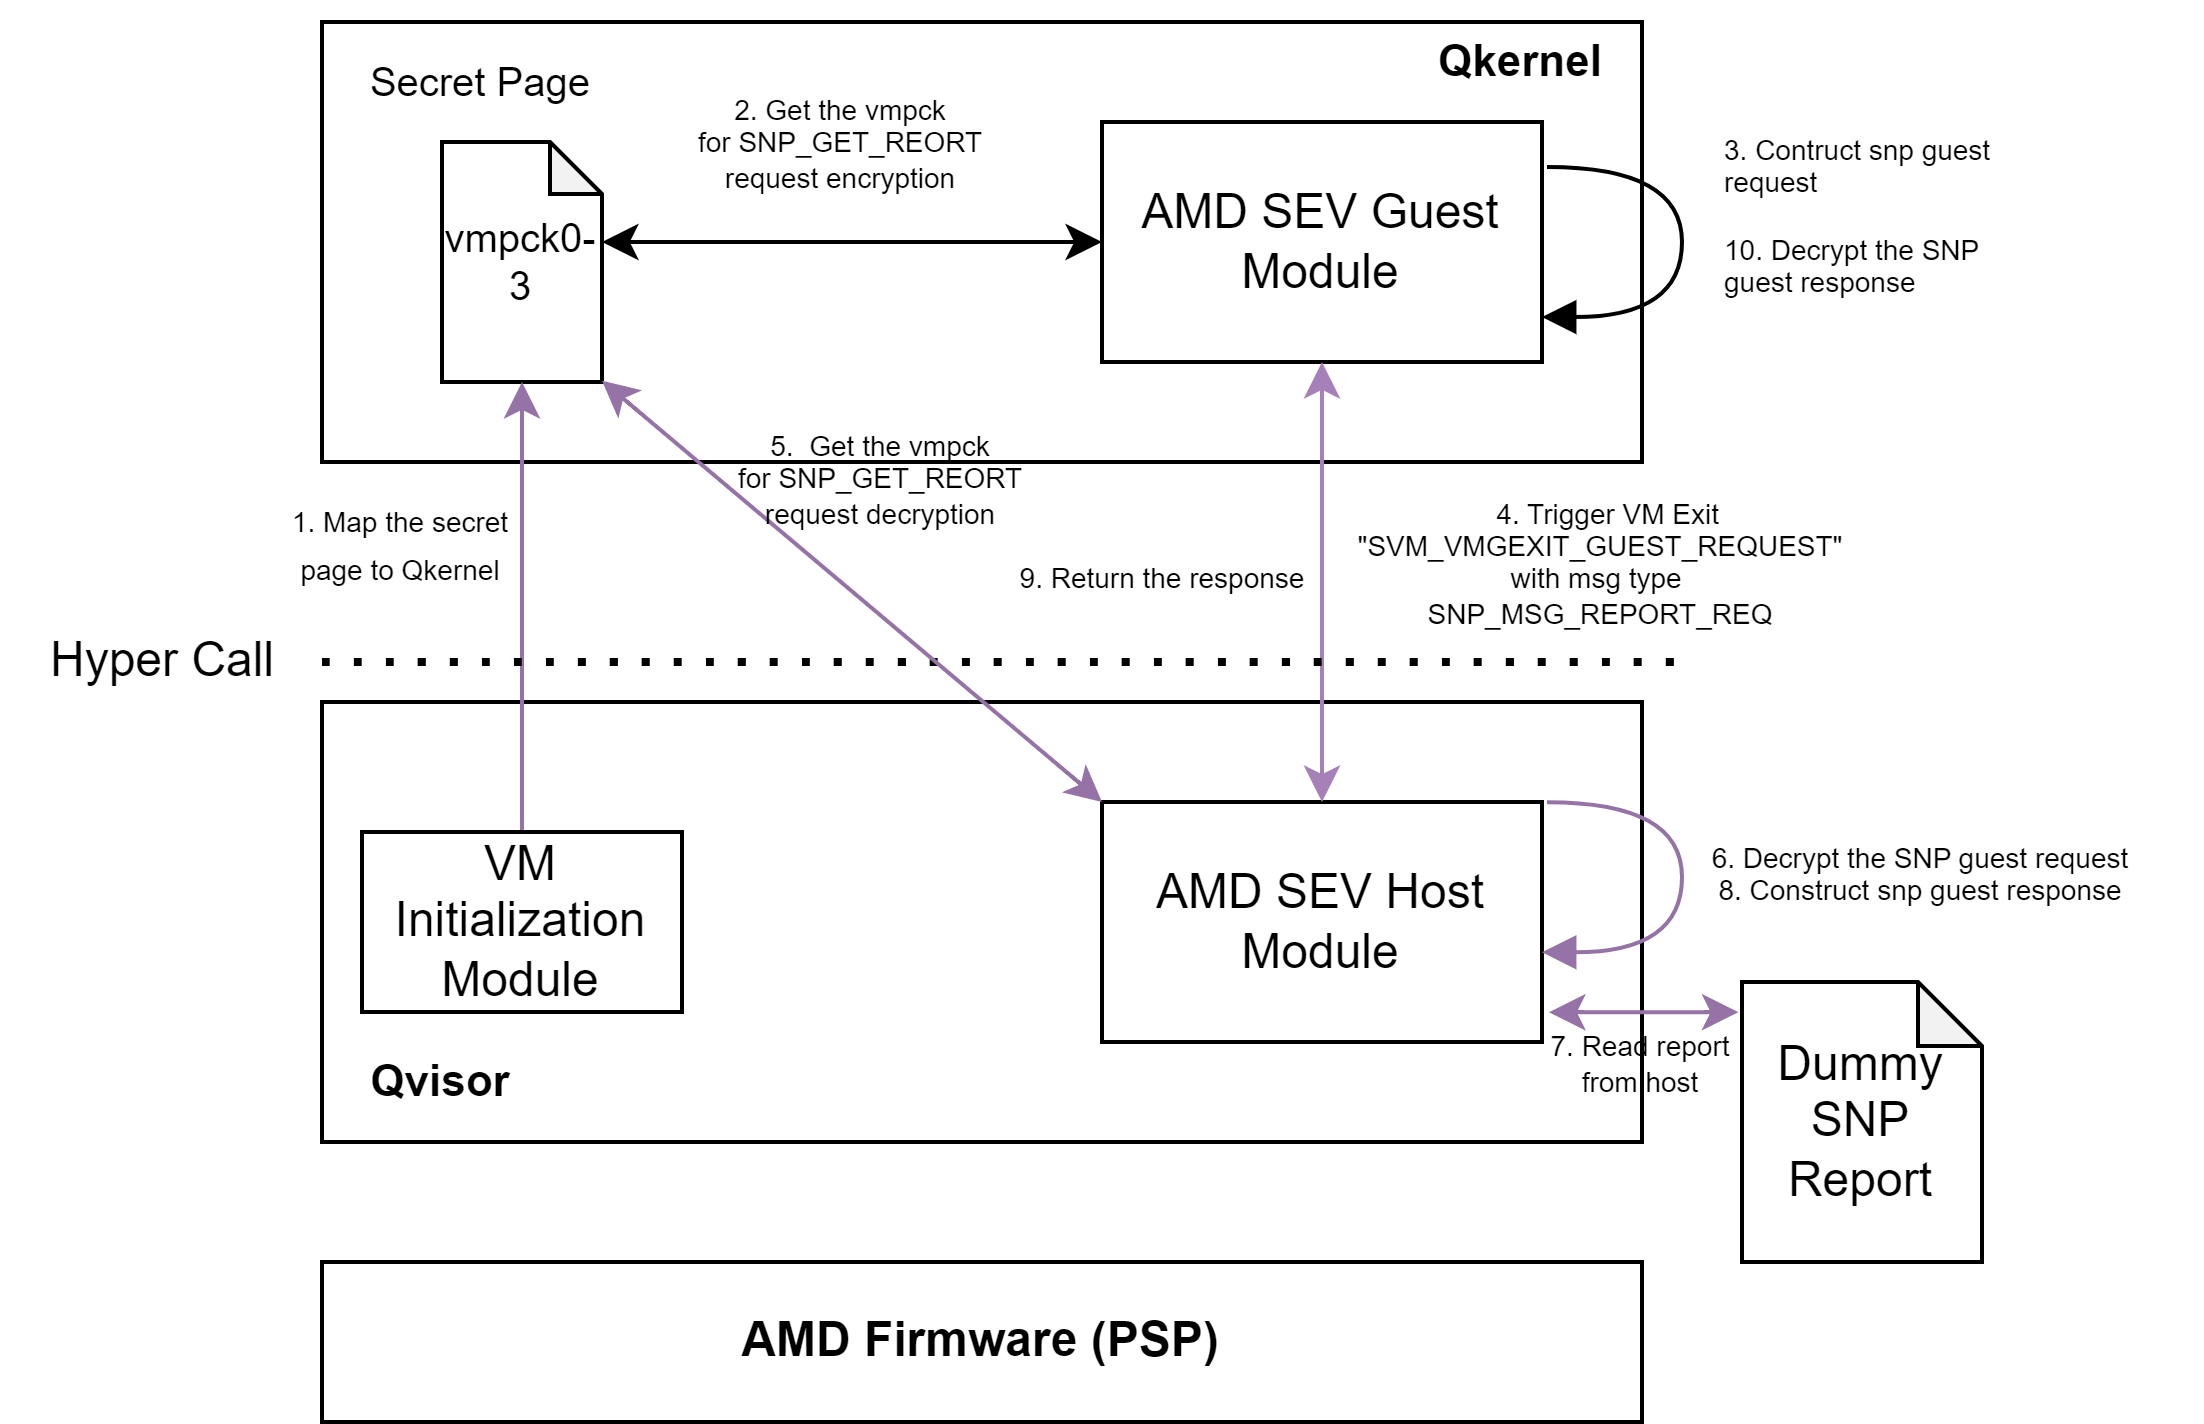
\includegraphics[width=0.8\textwidth]{images/amd_snp_driver.png}
    \caption[Attestation Driver Workflow]{Attestation Driver Workflow}
    \label{fig:amd_snp_driver}
\end{figure}

To simulate the process above, as shown in Figure~\ref{fig:amd_snp_driver}, Qvisor's VM initialization module initializes a secret page during the virtual machine's creation process. This page is mapped to shared memory between Qvisor and Qkernel. When the \acrshort{CVM} requests an attestation 
report, the attestation driver creates an  SNP request using a \texttt{VMPCK} on the secret page. This request is relayed to the AMD SEV SNP firmware emulation module in Qvisor via the hypercall \emph{SVM\_VMGEXIT\_GUEST\_REQUEST}. This module emulates SNP firmware. It will decrypt the request 
using the \texttt{VMPCK} on the page. A dummy report is then retrieved from the disk and tweaked according to the attestation driver's requirements for the user-defined field. Subsequently, the SNP module encrypts the altered report with \texttt{VMPCK} and returns it to the attestation driver as 
the SNP response payload. The attestation driver can decrypt the response and retrieve the report using \texttt{VMPCK}.

This driver provides the API in Listing~\ref{lst:Attestation_driver}. It takes user-defined data and returns a report serialized as a JSON string. The user-defined data is added to the custom field of the report. Returning a string instead of a specific report allows extending this driver to 
support multiple \acrshort{TEE}s. Specifically,  when it receives a request to generate a report, it will generate a report in different formats depending on the type of \acrshort{TEE}. Then, it will serialize this report into a string and return it to the requestor. The requestor can deserialize 
this string to get the specific report according to the \acrshort{TEE} type.

\begin{lstlisting}[language=rust, caption= API of attestation driver, label={lst:Attestation_driver}]
pub fn get_report(&mut self, report_data: String) -> Result<String>   
\end{lstlisting}

\subsection{Runtime Attestation Support}
The API of the runtime attestation support is shown in the Listing~\ref{lst:runtime_attestation}. A new system call with id 451 is added to the Qkernel for runtime attestation support. The \emph{SysAttestationReport} function is the handler for this system call. It accepts parameters, 
user-defined data, data length, and \emph{Request} and returns a report to the application. Here, the \emph{Request} allows the application to specify the desired report type.

\begin{lstlisting}[language=rust, caption= Interface for accessing the file type secrets, label={lst:runtime_attestation}]

pub struct Requst {
    pub software_based_report_requered: bool,
    pub use_user_provided_signing_key: bool,
    pub signing_key_length: usize, 
    pub signing_Key: [u8; 4096],  
}

pub struct Report {
    //  AMD SNP: 2, TDX: 3, Software based: 4
    pub tee_type: u64,
    pub report_length: u64,
    //  AMD SNP REPORT has 1183 bytes, INTEL TDX report has 1024 bytes
    pub report: [u8; 4096],  
}

pub fn SysAttestationReport(task: &mut Task, args: &SyscallArguments) -> Result<i64>      
\end{lstlisting}

\emph{SysAttestationReport} can generate software or hardware reports. In order to return a report of any type, the function serializes a report as a JSON string. It then converts the string into a byte array and embeds the array in the \emph{report} field of the \emph{Report} structure. After that, 
\emph{SysAttestationReport} copies the \emph{Report} structure to the address specified by the application. The application can get the length of the report character array from the \emph{report\_length} in the \emph{Report} structure. After converting the report character array to a string, 
the type of the report can be determined from the \emph{tee\_type} field, and the string can then be deserialized to an appropriate report. The format of the software report has been described in Section~\ref{sec:runtime_attesation}, while the format of a hardware report depends on the 
\acrshort{TEE} type.

\section{Software Measurement Manager}
\label{sec:impl_measurement}

This section describes how the software measurement manager measures data loaded from the host, such as dynamic link libraries, binary files, etc., and obtains shield startup hash, runtime hashes, application startup reference hash, and application restart hash.

\subsection{Binary Measurement}

\begin{figure}[!htb]
    \centering
    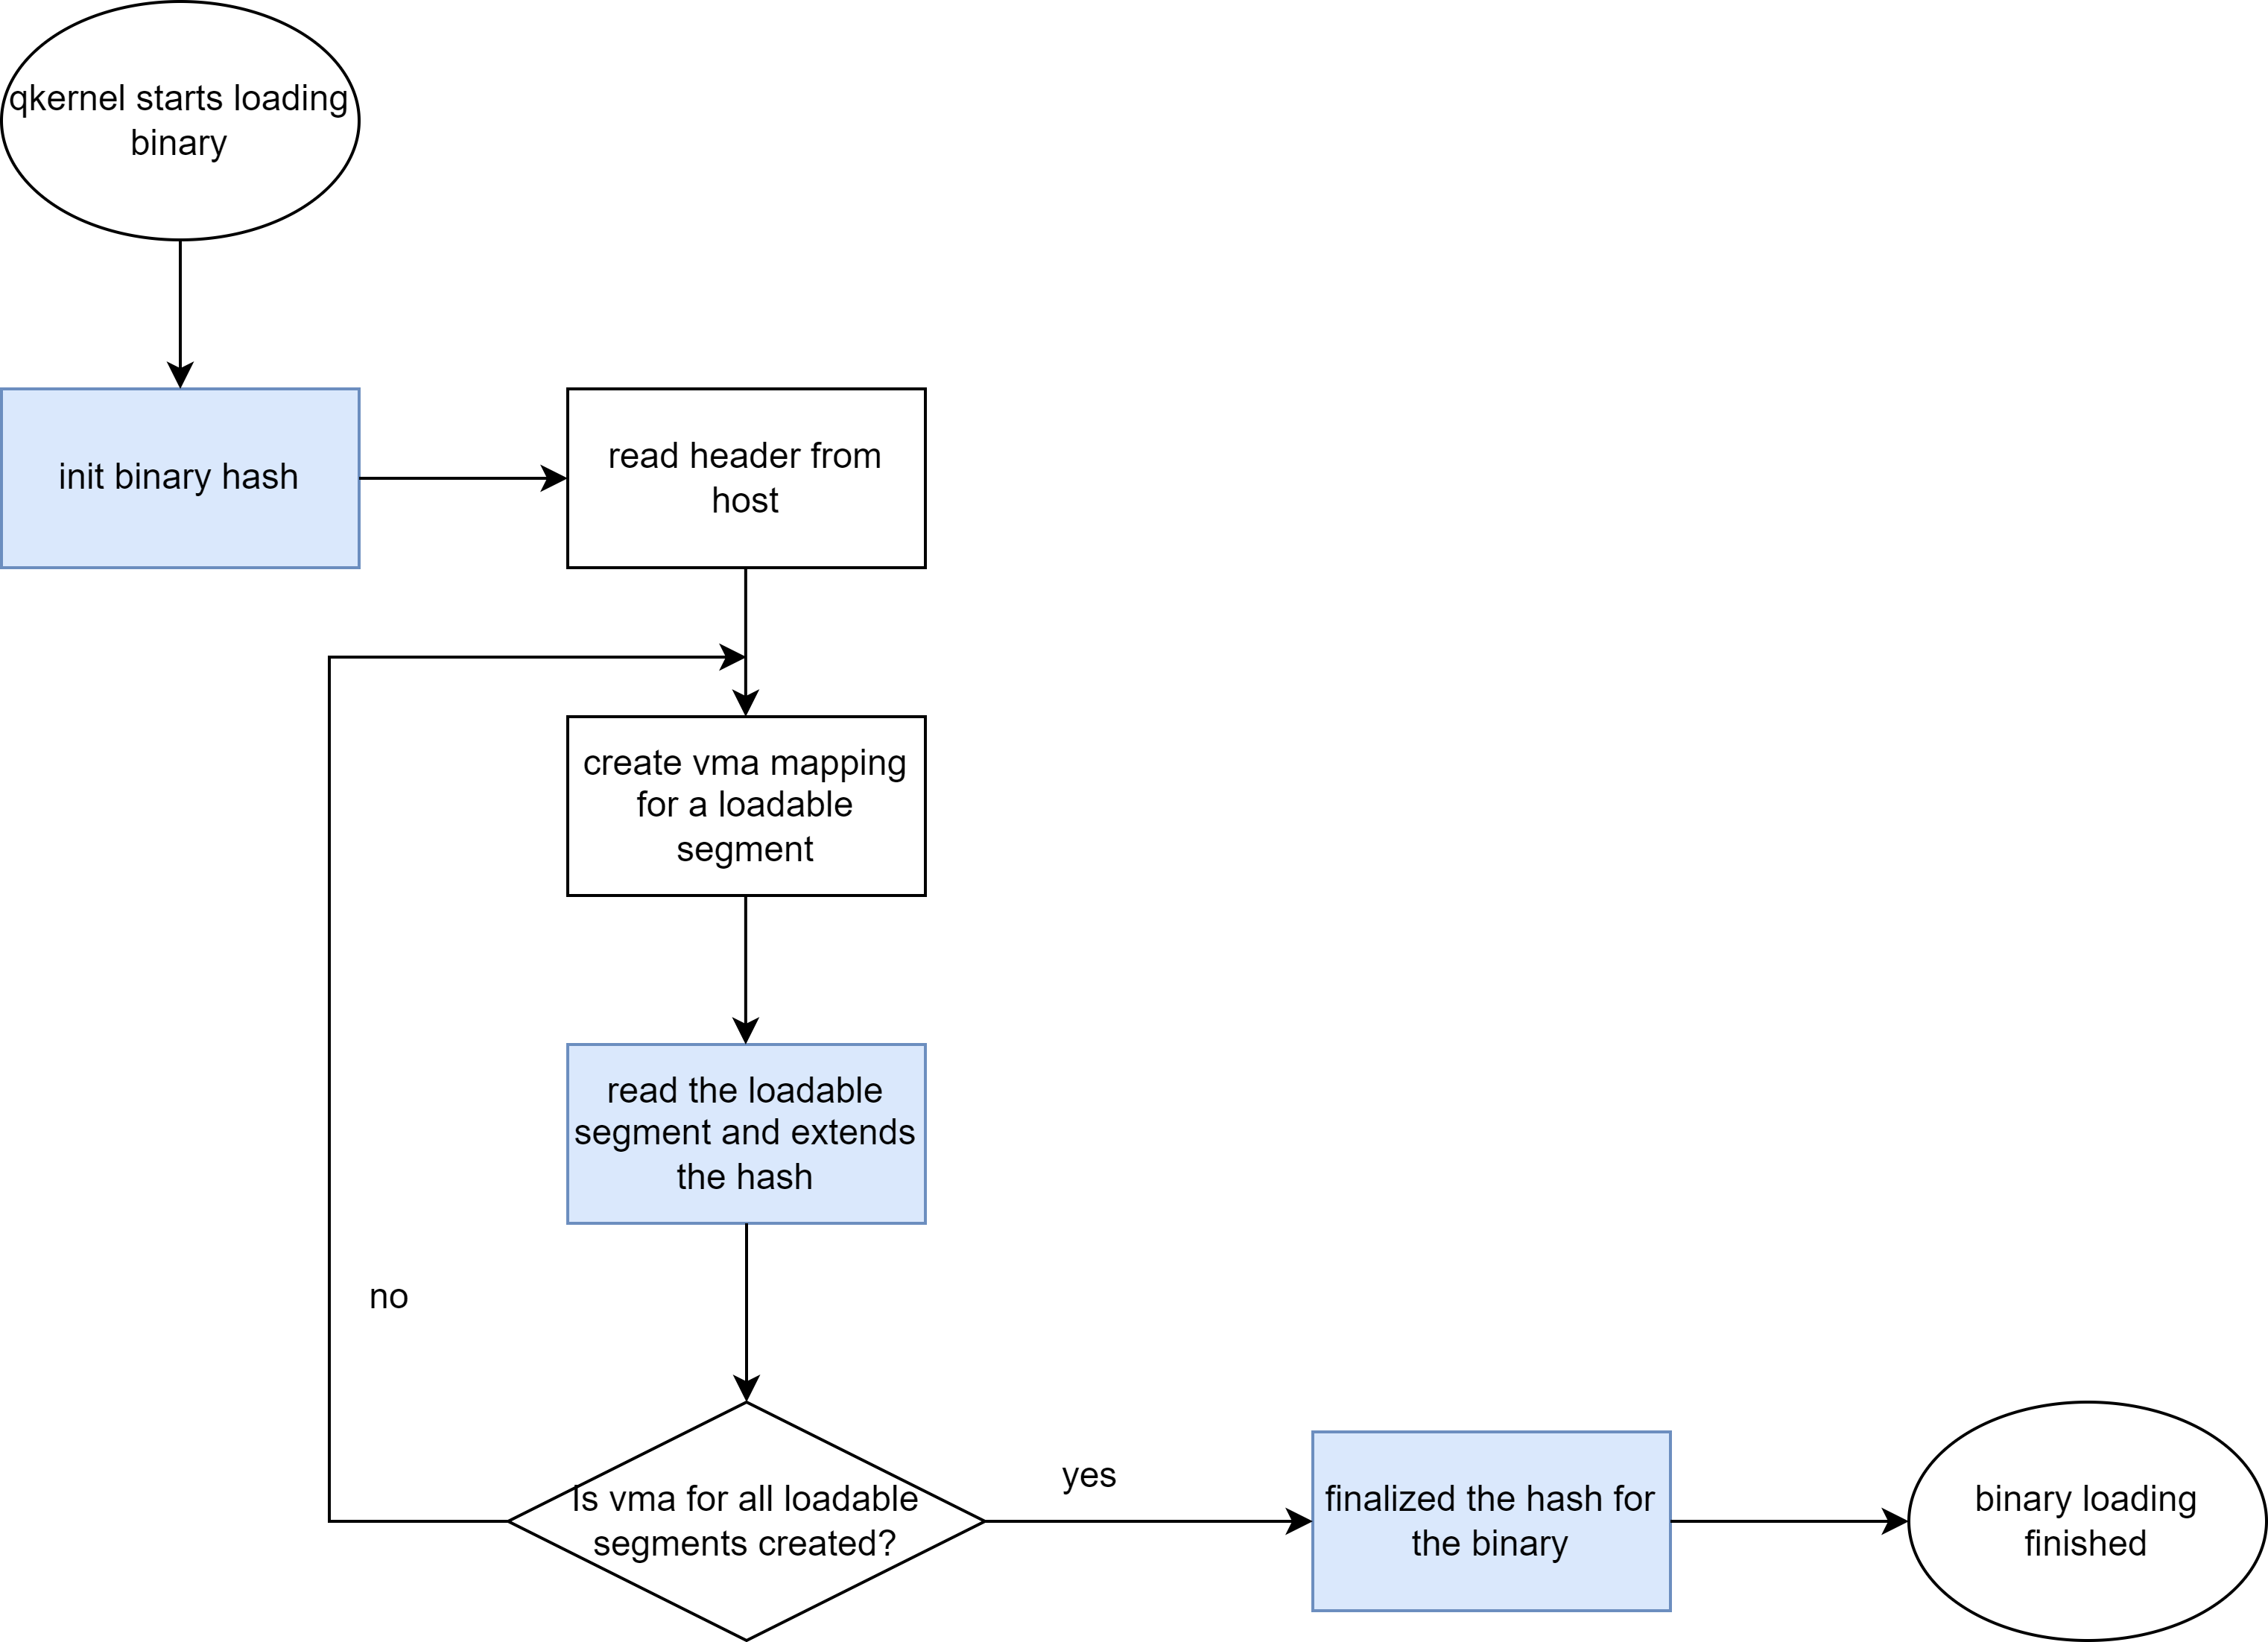
\includegraphics[width=0.8\textwidth]{images/measure_binary.png}
    \caption[Binary measurement workflow]{Binary measurement workflow}
    \label{fig:binary_measurement}
\end{figure}

Figure~\ref{fig:binary_measurement} depicts the workflow of binary measurement. Before the Qkernel loader loads a binary, the manager initializes a hash and saves it in a BtreeMap. While the binary is being measured, the manager can find the hash value using the binary name and extend it. 
As discussed in Section~\ref{sec:app_binary_loading}, the loader loads a binary by reading the binary header and creating a \acrshort{VMA} for each loadable segment. After creating a \acrshort{VMA}, the manager reads the guest virtual address range of the \acrshort{VMA} and extends the binary's hash 
utilizing the data read. The read operation will trigger page fault processing, which loads the appropriate data into guest memory (refer to Section~\ref{sec:app_binary_loading}). After the loader completes the creation of \acrshort{VMA}s for all loadable segments, the manager can obtain the 
binary measurement from the BtreeMap.




\subsection{Shared Library Measurement}

The workflow for shared library measurement is depicted in Figure~\ref{fig:measure_load_shared_libarart}. When the interpreter begins to load a dynamic library, it initiates the open system call to obtain the file descriptor for the shared library. The Qkernel \texttt{open} system call 
handler processes the open system call and determines whether a file is a shared library by checking its suffix (i.e., .so). If so, the handler notifies the software measurement manager to initialize a hash for the shared library, which is then stored in a BtreeMap. The manager can 
retrieve the hash from the map and extend it based on the library's name.


\begin{figure}[!htb]
    \centering
    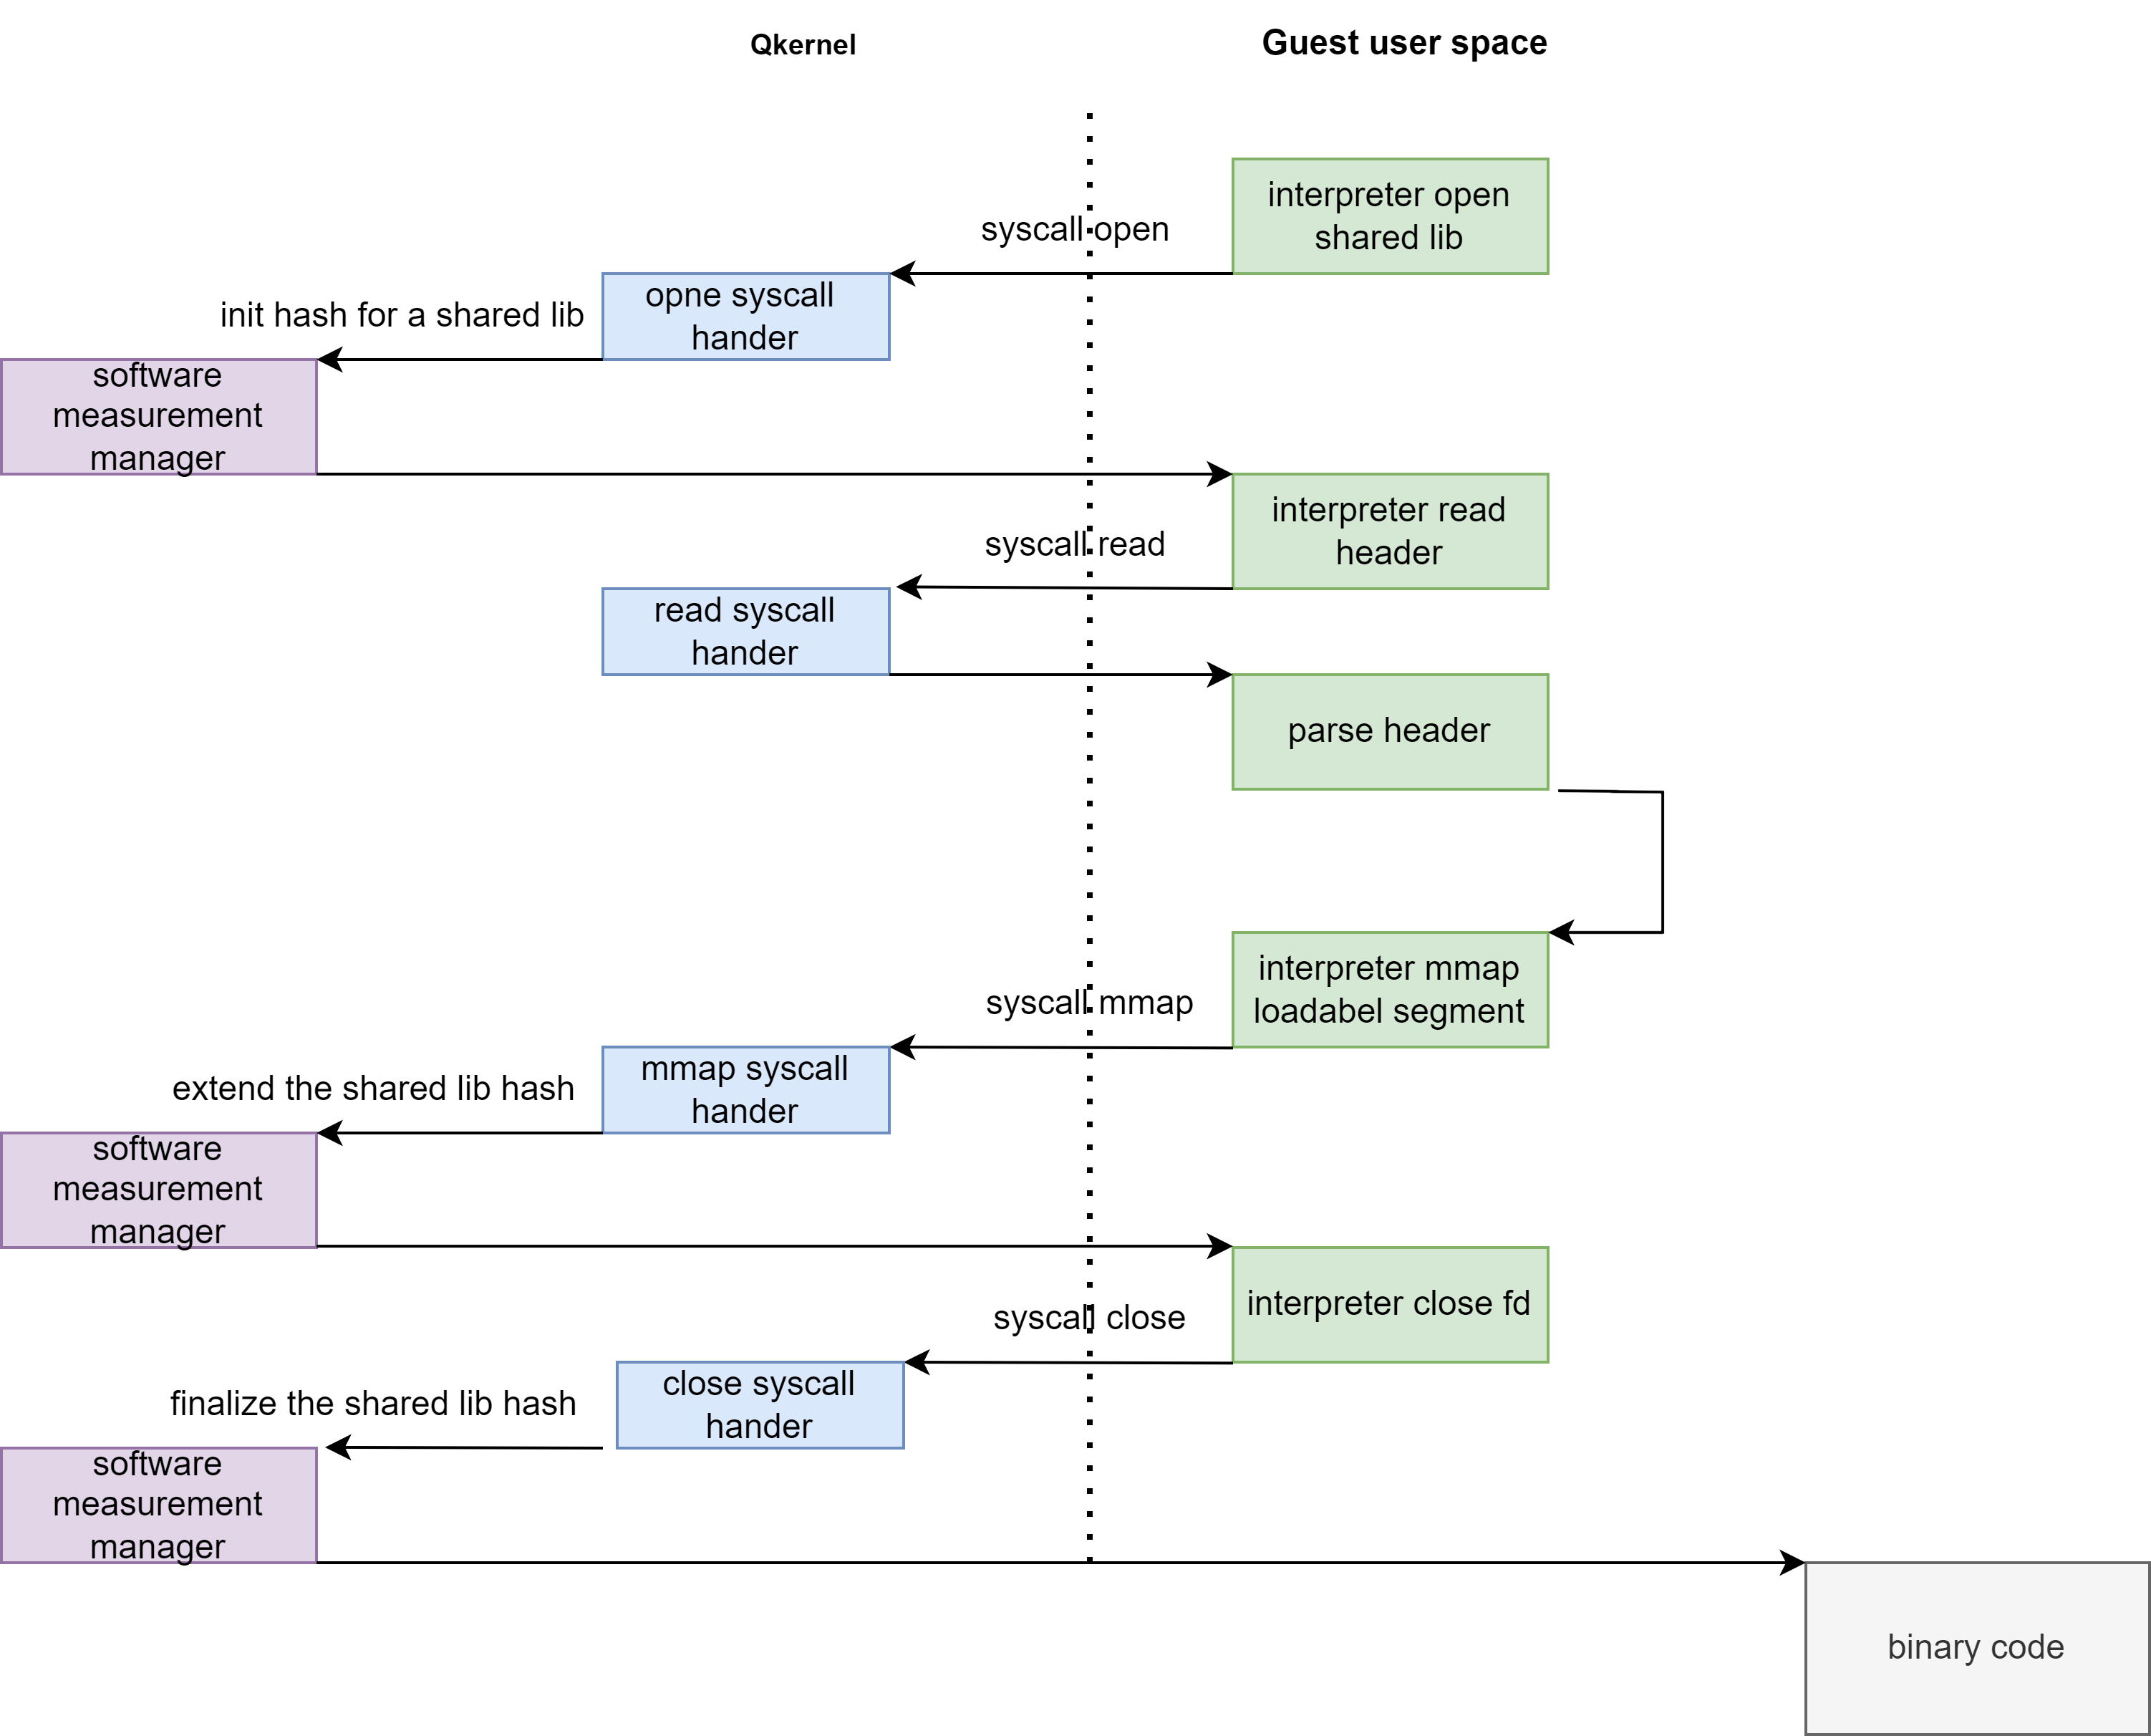
\includegraphics[width=0.8\textwidth]{images/measure_load_shared_libarart.png}
    \caption[Shared library measurement workflow]{Shared library measurement workflow}
    \label{fig:measure_load_shared_libarart}
\end{figure}

Once the open system call completes, the interpreter uses the read system call to read the library's header and find the loadable segments of the library. It then calls the mmap system call to create a \acrshort{VMA} for each segment. After the Qkernel \texttt{mmap} system 
call handler creates a \acrshort{VMA}, it invokes the software measurement manager. The manager will read the guest virtual memory range of the \acrshort{VMA} and extends the library's hash in the BtreeMap. As analyzed in Section~\ref{fig:measure_load_shared_libarart}, the read operation will cause 
the page fault handler to load the necessary data into the Qkernel. Since a shared library can have several loadable segments, the mmap system call can be invoked several times. The library's hash may thus be extended multiple times.


Measuring the loadable segments of a shared library is a challenge. Since the shared library is location-independent, the interpreter may map it to any location. The only requirement is that the Qkernel must make room for all the segments in their specified positions relative to the first segment. 
For this reason, the interpreter increases the mapping length to cover all the segments while mapping the first loadable segment. Because the mapping for all the segments might not be contiguous, the first \acrshort{VMA}'s virtual address range may be larger than the file size. This makes measuring 
the first segment difficult, as a \texttt{KVM segment fault} may be triggered if the software measurement manager reads the first \acrshort{VMA}'s address range directly. To avoid this, the software manager checks whether the \acrshort{VMA} size exceeds the file size of the shared library. 
If it does, the manager sets the measurement length to the file size of the shared library, which will cause the entire shared library to be measured. This way, the software manager can measure the first loadable segment and avoid the \texttt{KVM segment fault}.



After creating the last \acrshort{VMA}, the interpreter executes the close system call to release the shared library's file descriptor. The system call handler, in turn, notifies the software measurement manager that the library loading is completed. The  manager then obtains the measurement 
result of the shared library from the map. The manager will process the result differently depending on the library's loading timing, as discussed in Section~\ref{sec:Enclave_Runtime_Measurement}.
\subsection{Other Measurements}
The software measurement manager uses the SHA-512 hash function. This function accepts an array of bytes and returns a hash. Since the Qkernel configuration file is a structure, the software manager first serializes it into a JSON string and then converts it into a byte array. The array will 
be used as input to the hash function to extend the shield startup hash. The secret manager's public key is a byte array. After the software measurement manager reads it into the \acrshort{CVM} from the directory \textbf{/usr/local/secret\_manager\_cert.pem}, it can be used directly to extend 
the shield startup hash.

\subsection{Implementation Detail}
The data structure presented in Listing~\ref{lst:shared_Lib_measurement_implementation_detail} maintained the metadata for the software measurement manager. The variables \emph{is\_app\_loaded}, \emph{load\_app\_start}, and \emph{load\_app\_end} are employed to track the time (i.e., sandbox container creation, application creation, application runtime, 
and application recreation) measurements taken shown in Figure~\ref{fig:soft_ware_manager_meausrment}. The manager can decide what to do with the measurements based on these three variables. The variable \emph{runtime\_binary\_reference\_measurement} stores the reference measurements for the binaries 
and shared libraries loaded at runtime. The variable \emph{global\_measurement} is a hash that can track the host data measurements since the \acrshort{CVM} starts. Additionally, during program startup and restart, the manager utilizes the variables \emph{app\_binary\_ref\_measurement} and 
\emph{restart\_binary\_measurement} to track the measurement of binaries. Moreover, the variable \emph{shared\_lib\_measurements} and \emph{binary\_measurement} record the temporary hash values assigned to shared libraries and binarise during the measurement process, respectively. 
The manager can retrieve the corresponding hash by the file name and extend it accordingly.


\begin{lstlisting}[language=rust, caption= Interface for accessing the file type secrets, label={lst:shared_Lib_measurement_implementation_detail}]
pub struct SoftwareMeasurementManager {
    enclave_mode: EnclaveMode,
    is_app_loaded: bool,
    load_app_start: bool,
    load_app_end: bool,
    runtime_binary_reference_measurement:  BTreeMap<String, String>,
    global_measurement : String,
    enclave_ref_measurement: String,
    shared_lib_measurements: BTreeMap<String, String>,
    binary_measurement:  BTreeMap<String, String>,
    app_binary_ref_measurement : String,
    restart_bianry_measurement : String,
    startup_shared_lib_measurement_results:  BTreeMap<String, String>,
    restart_shared_lib_measurement_results:  BTreeMap<String, String>,
}
\end{lstlisting}

Since the order in which shared libraries are loaded may vary each time the application starts, the software measurement manager uses BTreeMap to record the measurement results for each shared library loaded during application startup and restart, i.e., \emph{startup\_shared\_lib\_measurement\_results} 
and \emph{restart\_shared\_lib}. As the Qkernel might initiate multiple processes during application startup to establish the application environment, a shared library can be loaded and measured multiple times. Therefore, when repeated measurements are made on a shared library, the manager compares 
the measurement stored in BTreeMap with the hash obtained when the library is repeatedly loaded. If there is a difference between the two, the manager will trigger a panic.


After the initial application setup, the manager generates a shield startup hash using the measurements stored in \emph{global\_measurement} and \emph{startup\_shared\_lib\_measurement\_results}. This hash is stored in the variable 
\emph{enclave\_ref\_measurement} as the \emph{shield startup hash}. The ordering of BTreeMap ensures that the generated shield startup hash is consistent each time.

The application startup reference hash generally refers to the measurements stored in \emph{variable app\_binary\_ref\_measurement} and \emph{startup\_shared\_lib\_measurement\_results}, whereas the application restart measurements involve the measurements stored in 
variable \emph{restart\_binary\_measurement} and \emph{restart\_shared\_lib\_measurement\_results}. When the application is restarted, the manager first compares the \emph{app\_binary\_ref\_measurement} with the \emph{restart\_binary\_measurement}. This guarantees that the binaries loaded during 
the application restart and initial startup are identical. Subsequently, a comparison is made between the measurements stored in \emph{startup\_shared\_lib\_measurement\_results} and \emph{restart\_shared\_lib\_measurement\_results} for the shared libraries. This verification ensures that all 
shared libraries loaded during application restart are consistent with those loaded during the initial application startup.



\section{EXEC Checker}
\label{sec:impl_exec}
The EXEC checker provides the Quark agent with the API shown in Listing~\ref{lst:exec_Cheker}. This function checks EXEC requests for legitimacy and handles session allocation or policy update requests from privileged users. It returns true if the EXEC request is legitimate and false if not. 
The \emph{ExecAuthenAcCheckArgs} contains the metadata required to create an EXEC process. In particular, the \emph{args} in \emph{ExecAuthenAcCheckArgs} is an array of strings containing the command to be executed and its arguments. If the request is privileged, the array \emph{args} is encoded 
using the schema discussed in Section~\ref{sec:design_prptect_privileged_request}

\begin{lstlisting}[language=rust, caption= API of EXEC checker, label={lst:exec_Cheker}]
pub struct ExecAuthenAcCheckArgs {
    pub exec_id: String,
    pub args: Vec<String>,
    pub env: Vec<String>,
    pub cwd: String,
    pub req_type: ExecRequestType,
}
pub fn exec_req_authentication (exec_req: ExecAuthenAcCheckArgs) -> bool
\end{lstlisting}

The workflow of the function is illustrated in Figure~\ref{fig:exec_req_authentication_flow_chart}. Initially, it determines the privilege level of the request by examining whether the first element of the array \emph{args} matches the keyword \texttt{Privileged}. If it does, the function 
validates and decrypts the encrypted payload in the array. Subsequently, it verifies the legitimacy of the request's session and counter. If these components are deemed illegitimate, the function returns false. It then identifies whether the request is a session assignment or policy update request 
using the methods described in Section~\ref{subsec:design_policy_session_update}. In the case of a typical Linux command, the function checks its legality based on the policy. Specifically, it first confirms if the command is included in the command allowlist. If it is, the function checks if the 
directory allowlist incorporates the path-like string found in the command's arguments. Notably, for a no-arguments command, the function verifies if the current execution directory of the command is present in the directory allowlist. For non-privileged commands, the function only evaluates 
their legality based on the policy. The algorithm for the command's arguments verification can be found in Section~\ref{sec:design_EXEC_Requests}. If a command meets the policy criteria, the function saves the EXEC request's command and argument in plaintext. The Quark agent can then employ 
the EXEC ID to retrieve a legitimate EXEC request's metadata and create the corresponding process.

\begin{figure}[!htb]
    \centering
    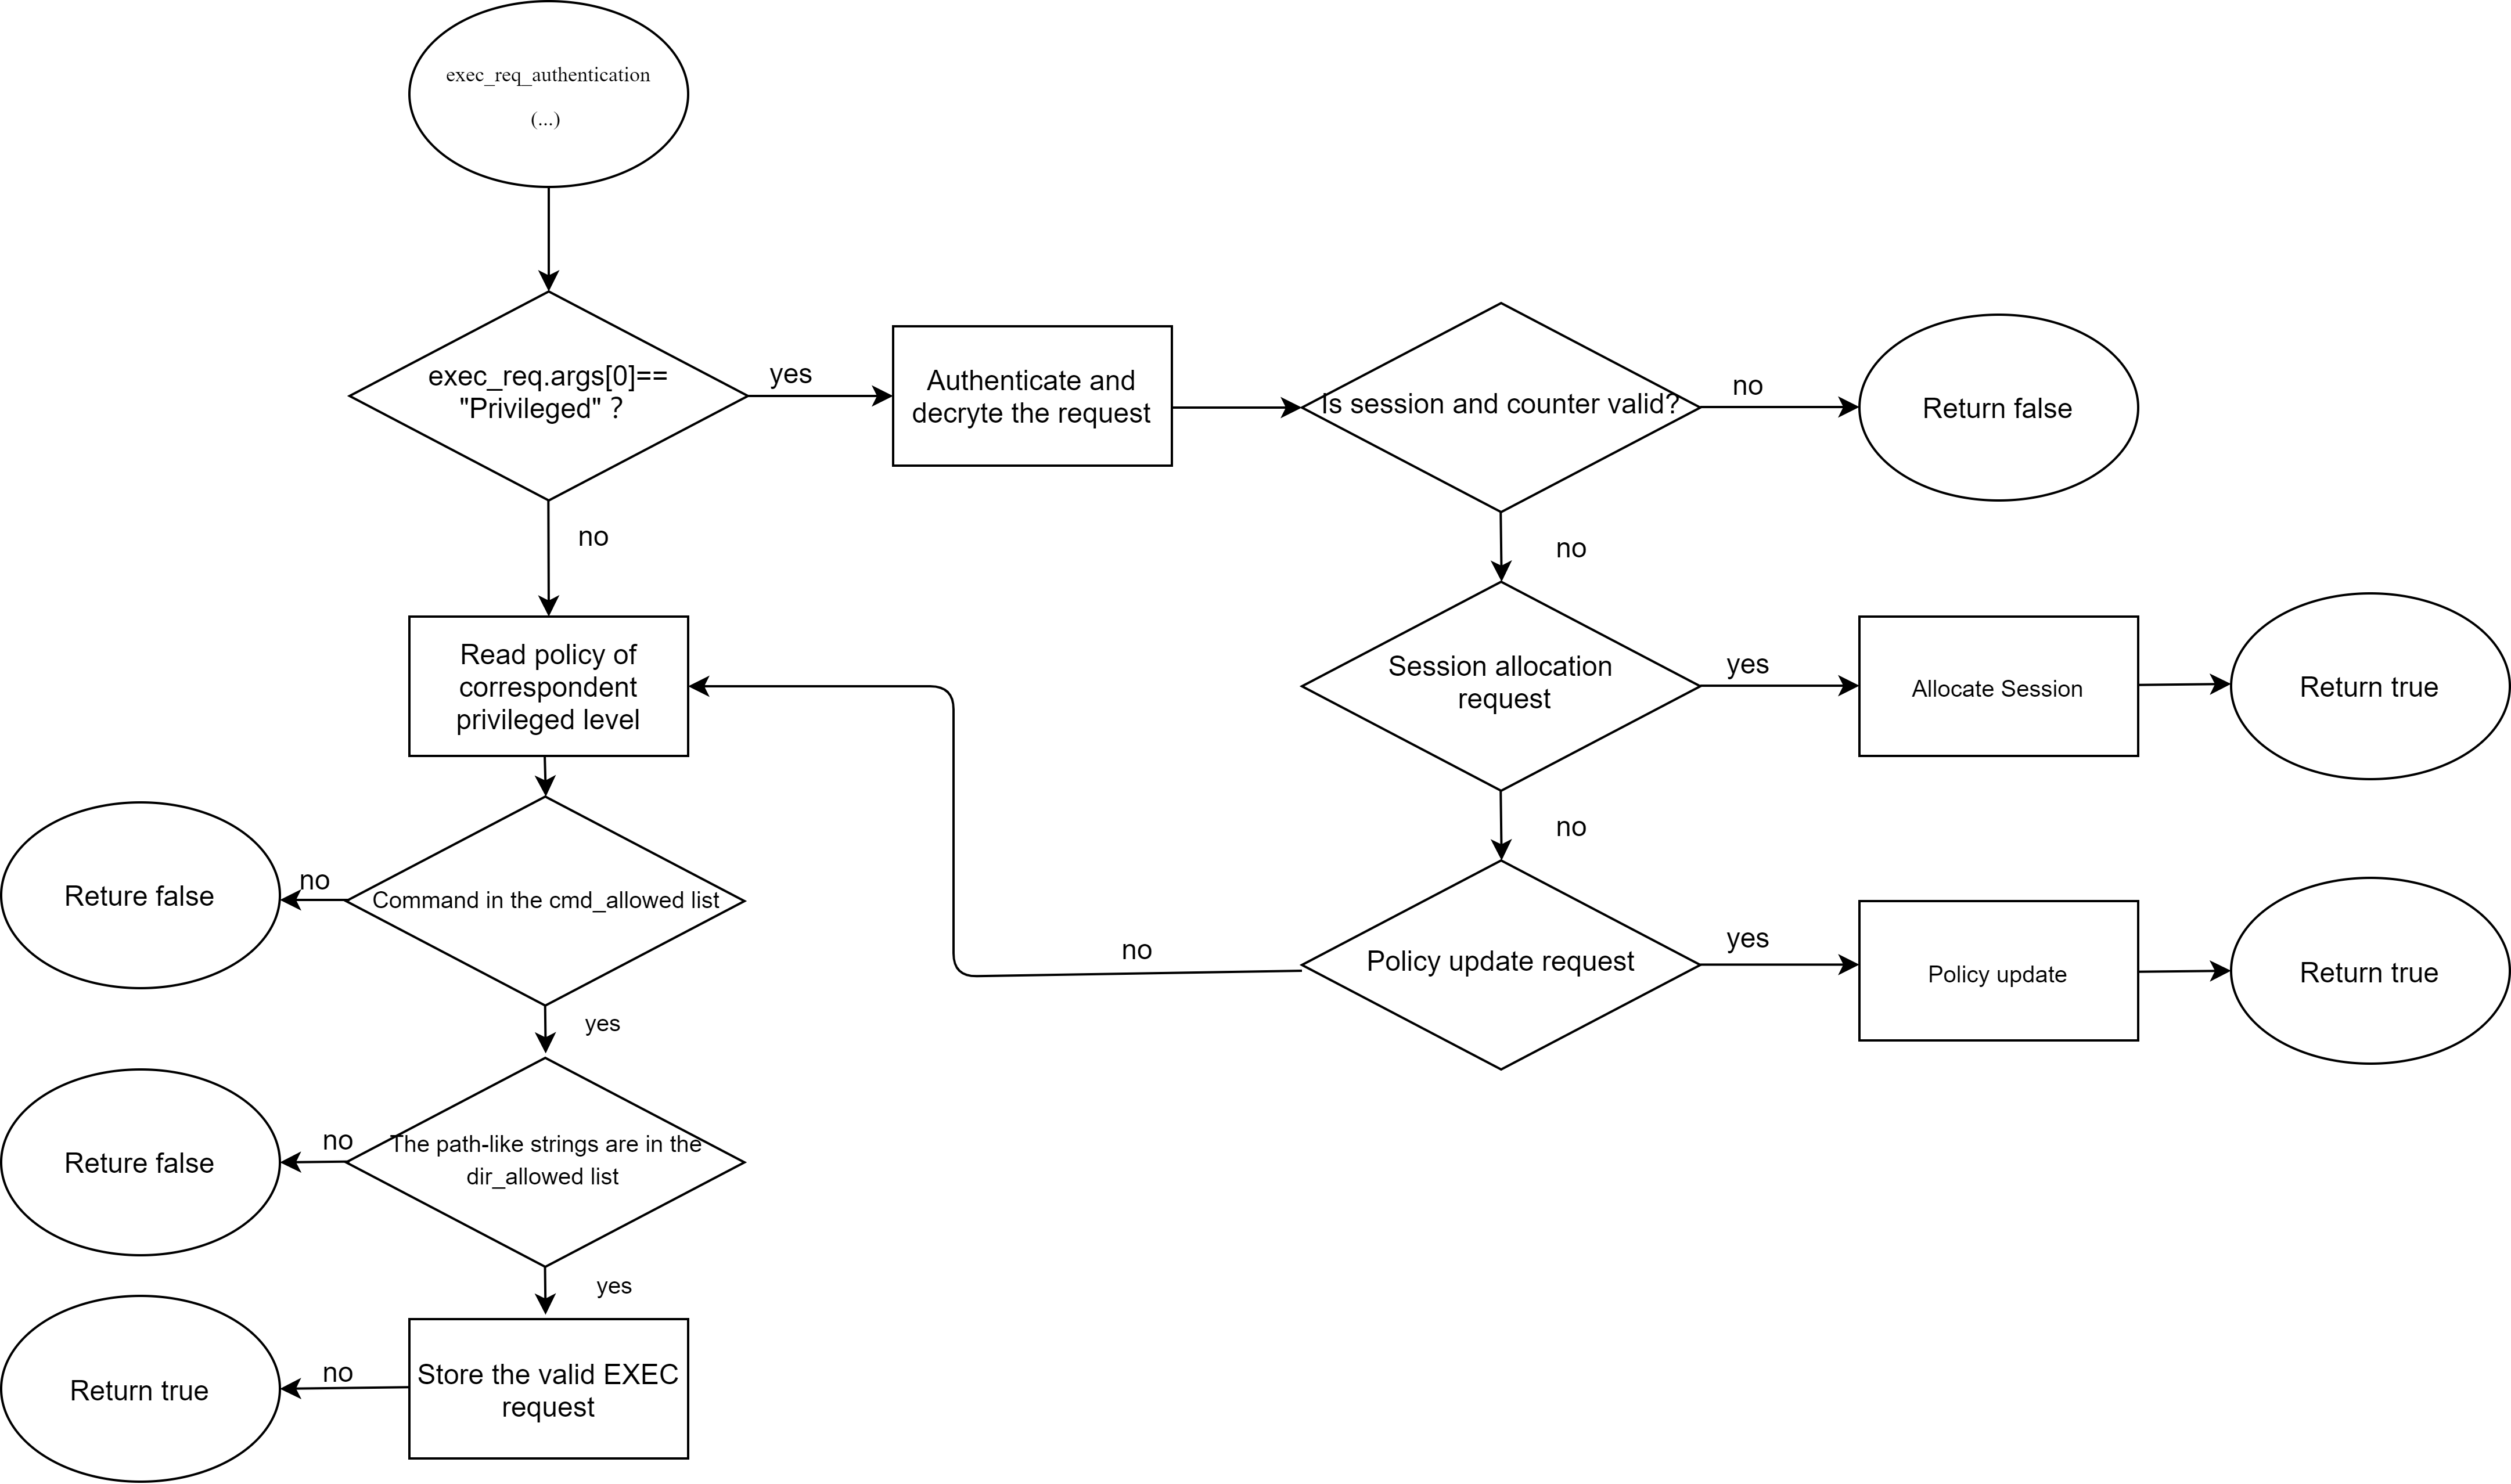
\includegraphics[width=0.8\textwidth]{images/exec_req_authentication_flow_chart.png}
    \caption[EXEC cheker workflow]{EXEC cheker workflow}
    \label{fig:exec_req_authentication_flow_chart}
\end{figure}

\section{STDIO Protection}
\label{sec:impl_STDIO}

\subsection{Inode Tracker}
The data structure \emph{InodeTracker} in Listing~\ref{lst:Inode_Tracker} records information about a file descriptor that represents a process’s STDIO. It maintains a map where the key is the inode id, and the value contains metadata related to the process. 
The detail of the data structure can be found in Section~\ref{sec:design_Distinguish_io}


\begin{lstlisting}[language=rust, caption= API of Inode Tracker, label={lst:Inode_Tracker}]
pub struct InodeTracker {
    inode_track: BTreeMap<u64, TrackInodeType>,
} 
\end{lstlisting}

\subsection{Non-interactive process STDIO Protection}
\begin{lstlisting}[language=rust, caption= API of normal IO shield, label={lst:Normal_IO}]
fn encrypNormalIOStdouterr (&self, src: DataBuff, inode_id: u64) -> Result<DataBuff>
\end{lstlisting}
The function in Listing~\ref{lst:Normal_IO} encrypts STDOUT and STDERR for non-interactive processes. It accepts data written to STDOUT or STDERR and the inode id corresponding to the STDOUT or STDERR file descriptor. Depending on the shield policy and the stored metadata in the \emph{InodeTracker}, 
the function encrypts the data using the method specified in Section~\ref{sec:design_non_interactive_stdio}. Subsequently, it returns the encrypted data to Qkernel. Qkernel then sends encrypted data out via Qcall.



\subsection{Interactive process STDIO Protection}
\begin{lstlisting}[language=rust, caption= API of system call interceptor, label={lst:Termianl_IO}]
fn termianlIoEncryption(&self, src: &[IoVec], task: &Task,  inode_id: u64) -> Result<(Vec::<IoVec>)
\end{lstlisting}
Like the \emph{encrypNormalIOStdouterr} function, the function in Listing~\ref{lst:Termianl_IO} is responsible for encrypting the STDOUT and STDERR of interactive processes. This ensures that the logs of the interactive application are encrypted, as discussed in Section~\ref{subsec:design_terminal}.

\section{System Call Interceptor}
\label{sec:impl_interceptor}
The three functions in the Listing~\ref{lst:Interceptor} are responsible for updating the interceptor’s policy at runtime, initializing the interceptor’s policy at \acrshort{CVM} startup, and determining whether a system call is allowed. When the interceptor operates in \texttt{ContextBased} mode, 
the \emph{is\_guest\_syscall\_allowed} function utilizes the application process id stored in the structure \emph{GuestSyscallInterceptor} to identify whether a process is the application process. To prevent competition between the three functions accessing the interceptor's policy, the interceptor is 
protected by RwLock. Additionally, the \emph{BackEndSyscallInterceptorConfig} maintains a vector that contains the id of allowed system calls (allowlist). The \emph{is\_guest\_syscall\_allowed} function checks whether a system call's ID is present in this list to determine whether the system call 
is allowed. It is important to note that accessing this allowlist has an O(n) time complexity.

\begin{lstlisting}[language=rust, caption= API of system call interceptor, label={lst:Interceptor}]
static ref SYSCALLINTERCEPTOR:  RwLock<GuestSyscallInterceptor> = RwLock::new(GuestSyscallInterceptor::default());

pub struct BackEndSyscallInterceptorConfig {
    pub syscalls: Vec<u64>
…
}

pub struct GuestSyscallInterceptor {
    policy: BackEndSyscallInterceptorConfig,
    application_pid: i32,
}

pub fn syscall_interceptor_policy_update(policy: &BackEndSyscallInterceptorConfig) -> Result<()> 
pub fn syscall_interceptor_init(policy: BackEndSyscallInterceptorConfig) -> Result<()> 
pub fn is_guest_syscall_allowed(current_pid: i32, syscall_id: u64) -> bool
    
\end{lstlisting}


\section{Qlog Manager}
\label{sec:iml_qlog}
Listing~\ref{lst:Qlog} presents the API of the Qkernel log manager. The \emph{QlogManager} structure maintains the Qlog manager's policy, as shown in Listing~\ref{lst:shiled_policy_log}. The shielding layer uses the function \emph{qlog\_manager\_init} to initialize or update the policy. 
The function \emph{is\_log\_level\_allowed}  is invoked by 
the Qkernel logging system. It accepts the level of the log that currently needs to be printed. It returns true if the log level is the same or less than the log level specified in the policy. If this function returns false, the Qkernel logging system will not print the log message.

\begin{lstlisting}[language=rust, caption= API of Qlog manager, label={lst:Qlog}]
pub struct QlogManager {
    policy: QlogPolicy,
}
pub fn is_log_level_allowed(current_log_level: QkernelDebugLevel) -> bool
pub fn qlog_magager_init()   
\end{lstlisting}


\section{Summary}
This chapter explained how the design in Chapter~\ref{sec:design} was implemented. The next chapter will evaluate the performance and security of the system.


\cleardoublepage



%%% Local Variables:
%%% TeX-master: "diplom"
%%% End:

